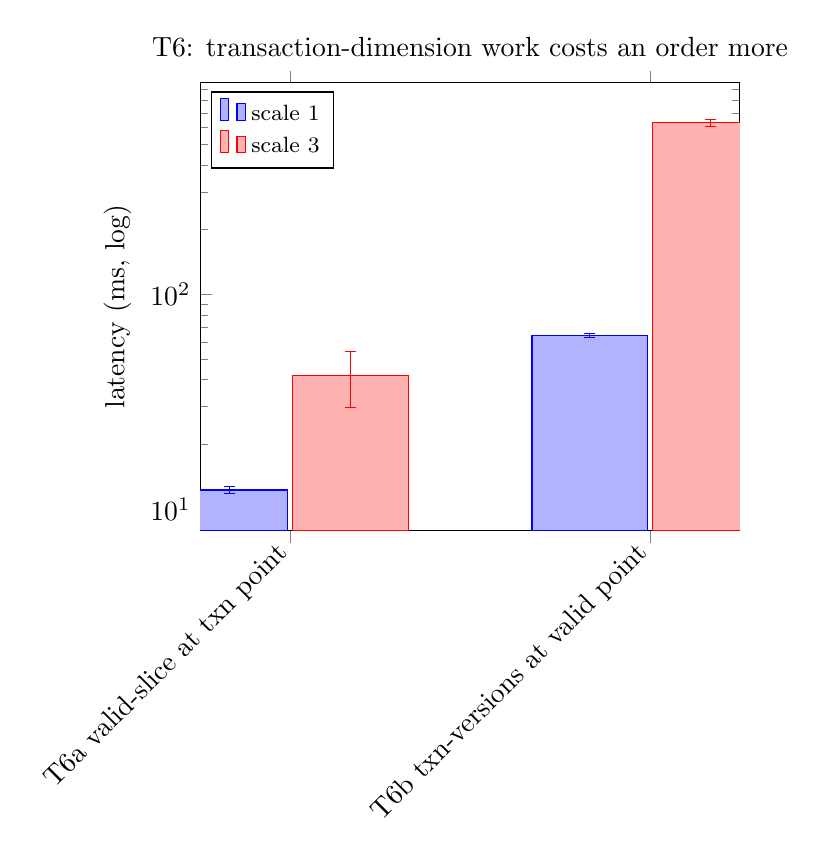
\begin{tikzpicture}
\begin{axis}[
  title={T6: transaction-dimension work costs an order more},
  ylabel={latency (ms, log)},
  ybar, bar width=0.32,
  enlarge x limits=0.25,
  ymode=log, log origin=infty,
  xtick=data,
  x tick label style={rotate=45,anchor=east},
  xticklabels={{T6a valid-slice at txn point},{T6b txn-versions at valid point}},
  legend style={at={(0.02,0.98)},anchor=north west,font=\footnotesize},
  error bars/y dir=both, error bars/y explicit,
]
  \addplot+[error bars/.cd,y explicit] coordinates {
    (1,12.244 ) +- (0.221,0.44 )
    (2,64.307 ) +- (1.382,1.174 )
  };
  \addlegendentry{scale 1}
  \addplot+[error bars/.cd,y explicit] coordinates {
    (1,41.999 ) +- (4.214,12.172 )
    (2,628.674 ) +- (3.386,21.267 )
  };
  \addlegendentry{scale 3}
\end{axis}
\end{tikzpicture}
{\footnotesize PRELIMINARY — non-reference hardware; medians of 5, bars show min/max. First readings, not reference figures (paper §5).\par}
